\documentclass[10pt,letterpaper]{article} 
\usepackage{tikz}
\usepackage{tools}
\usepackage{enumitem,caption}
\usepackage{listings}
\usepackage{xepersian}
\lstset{language=Python}
%\lstset{frame=lines}
%\lstset{caption={Insert code directly in your document}}
\lstset{label={lst:code_direct}}
\lstset{basicstyle=\footnotesize}

%\usepackage{graphicx}‎‎
%\usefonttheme{serif}‎
%\usepackage{ptext}‎
%\usepackage{xepersian}
%\settextfont{B Nazanin}
\usepackage{lipsum}
\setlength{\parindent}{0pt}
\newcommand{\pf}{$\blacksquare$}

\newcommand{\Span}{\text{Span}}
\newcommand{\NF}{\text{NF}}
\newcommand{\EDFA}{\text{EDFA}}
\newcommand{\ASE}{\text{ASE}}

\newcommand{\bns}{\textit{broadcast-and-select}  architecture}
\newcommand{\Bns}{\textit{Broadcast-and-select} architecture}

\newcommand{\rns}{\textit{route-and-select} architecture}
\newcommand{\Rns}{\textit{Route-and-select} architecture}

\newcounter{QuestionNumber}
\setcounter{QuestionNumber}{1}

\newcommand{\temp}{{\color{red}{temp}}}

\newcommand{\Q}{
\textbf{سوال \theQuestionNumber)}
\stepcounter{QuestionNumber}
}
\newcommand{\EX}{\Bbb E}
\newcommand{\nl}{\newline\newline}
\begin{document}
\large
\begin{center}
به نام او

میان ترم شبکه های مخابرات نوری

مدت زمان: 90 دقیقه
\hl
\end{center}

\Q

نحوه اتصال ورودی و خروجی هر المان نوری را می توان به صورت یک جدول مدل کرد که عنصر واقع در سطر $i$-ام و ستون $j$-ام این جدول، شماره پورت خروجی را نشان می دهد که طول موج $j$-ام از آن خارج می شود، هنگامی که روی پورت ورودی $i$-ام وارد این المان شده باشد. توجه داشته باشید که اگر طول موجی مالتی‌کست شده باشد، در جدول مربوطه بیش از یک پورت خروجی در یک خانه جدول قرار خواهد گرفت.

الف) تعیین کنید از بین سه جدول زیر، کدام یک مربوط به یک WSS دارای چهار پورت ورودی و چهار پورت خروجی است.

ب) جدول ورودی-خروجی یک splitter (که سیگنال را در پایانه های خروجی خود تقسیم می‌کند) را ترسیم کنید.

\begin{figure}[h]
\centering
\includegraphics[width=140mm]{Jadval.png}
\end{figure}

\newpage
\Q

مسئله ILP زیر را به کمک رسم ناحیه شدنی و تابع هدف حل کنید.

\[\begin{split}
&\text{minimize}\ \  x_1+x_2
\\& \text{to subject}
\\& \ \ \ \ \ \ x_1-2x_2\le 4
\\& \ \ \ \ \ \ 3x_2\le 6x_1+8
\\& \ \ \ \ \ \ 2x_2+4x_1\le 17
\\& \ \ \ \ \ \ x_2\le5
\\& \ \ \ \ \ \ x_1,x_2\in\mathbb{Z}
\end{split}\]

\newpage
\Q
در شبکه زیر به کمک الگوریتم های 
Dijkstra
و
Bellman-Ford،
کوتاه ترین مسیر بین نود های A و Z را بیابید. در صورتی که پاسخ این دو روش متفاوت است، تفاوت را به طور کامل توضیح دهید.

\begin{figure}[h]
\centering
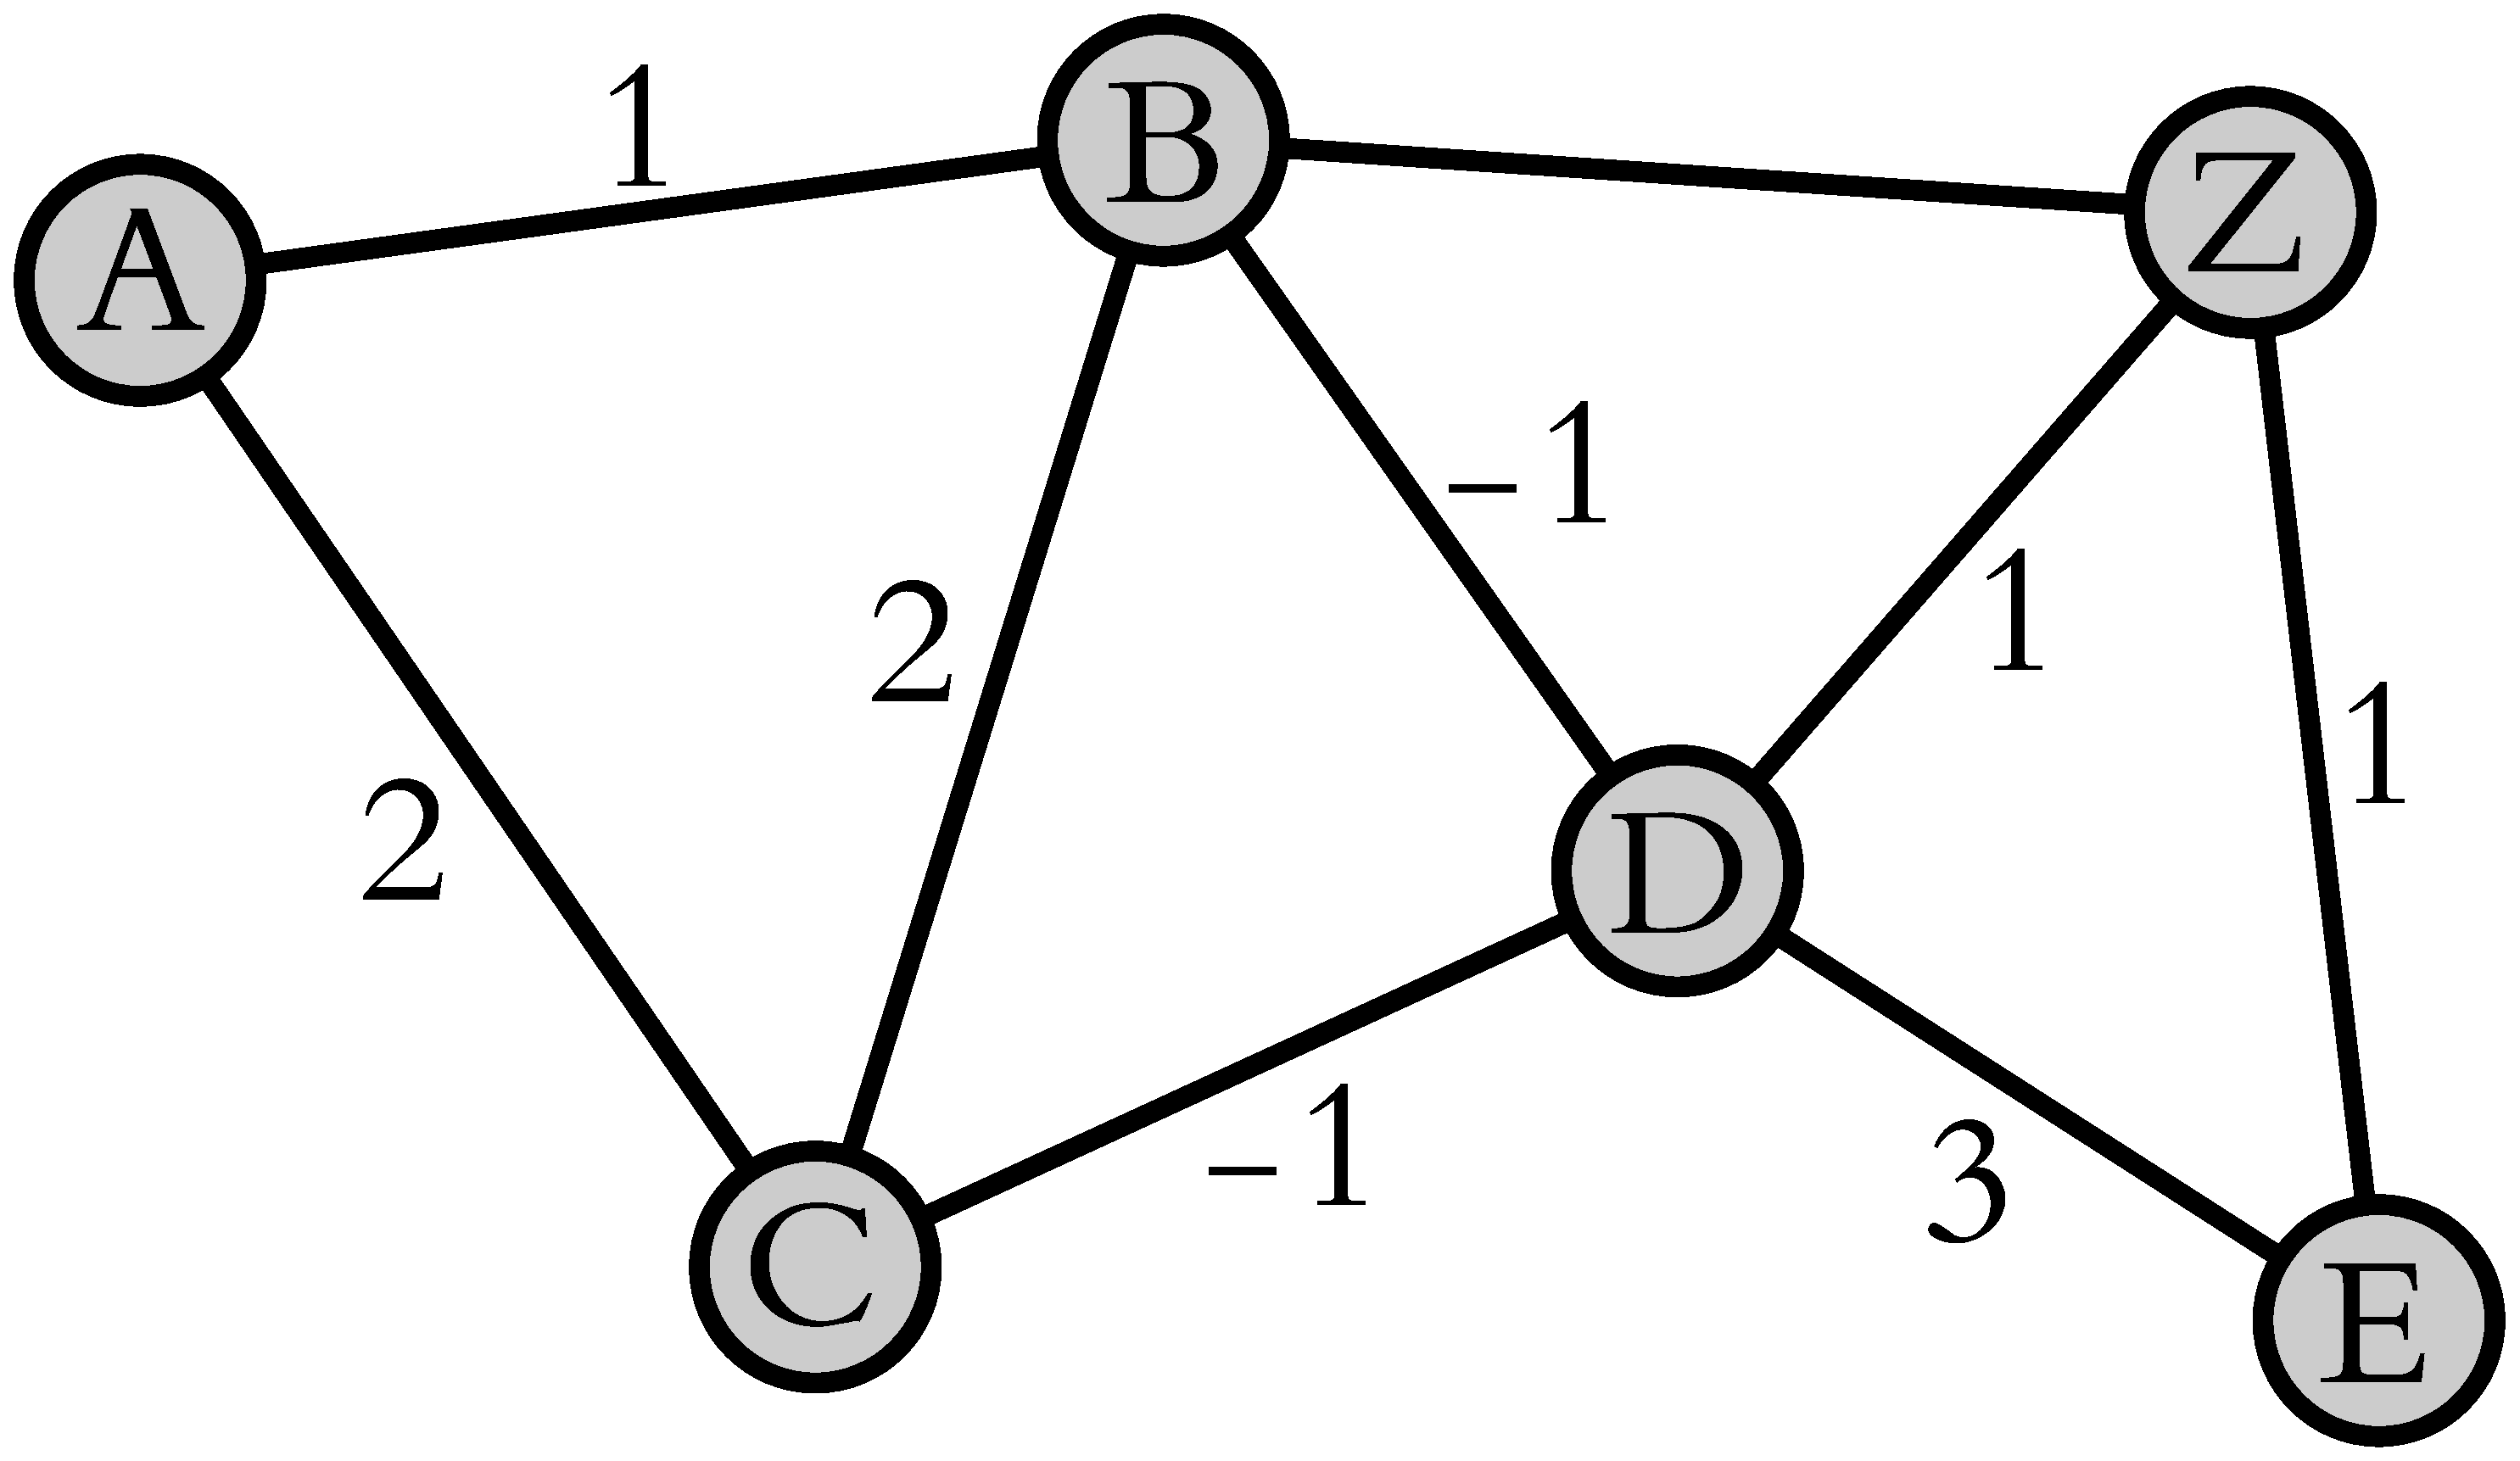
\includegraphics[width=70mm]{midterm_bell_dij}
\end{figure}

\newpage
\Q

یک لینک نوری متشکل از یک فیبر 80 کیلومتری با تضعیف 
$
0.22\text{dB/km}
$
 و دو تقویت کننده است که تقویت کننده طبقه اول از نوع Raman و طبقه دوم از نوع EDFA است. عدد نویز تقویت کننده Raman با هر 1dB افزایش در بهره آن، به صورت خطی 
$
0.3\text{dB}
$
 کاهش می یابد و عدد نویز آن به ازای بهره 10dB برابر 
$
21.5\text{dB}
$
 است. عدد نویز EDFA نیز به طور مستقل از بهره آن برابر 6dB است. چنانچه حداکثر بهره تقویت کننده Raman برابر 15dB ، حداکثر بهره EDFA برابر 5dB و بهره لینک برابر 0dB باشد:

الف) مقادیر بهینه بهره های دو طبقه تقویت کننده های Raman و EDFA برای داشتن کمترین عدد نویز کلی لینک چقدر است؟

ب) فرض کنیم یک مسیر نوری شامل $N$ تا از لینک های فوق (با مقادیر بهینه به دست آمده برای بهره تقویت کننده ها در قسمت الف) است و SNR یک سیگنال نوری که از ابتدای این مسیر تا انتهای آن انتشار می یابد، می تواند حداکثر تا 33dB بدون اعمال regeneration افت کند. حداکثر مقدار $N$ جهت انتشار تمام-نوری (بدون regeneration) چقدر است؟

\newpage
\Q

در توپولوژی فیزیکی داده شده‌ی زیر، مسیرهای نوری با نقطه چین و اندیس 1 تا 9 مشخص شده اند. به کمک الگوریتم‌های first-fit و most-used به هریک از مسیر های نوری، طول موج اختصاص دهید. اگر هر لینک دارای حداکثر سه ظرفیت در طول موج های 
$
\lambda_1
$
،
$
\lambda_2
$
و
$
\lambda_3
$
 باشد، آیا در روشهای فوق مسیر نوری مسدود شده خواهیم داشت؟

\begin{figure}[h]
\centering
\includegraphics[width=120mm]{first-fit-most-used-midterm}
\end{figure}




\end{document}